% greyscaleCCA.tex
% black hole weather, feeding by chaotic cold accretion and self regulating feedback, greyscale
% standalone, compile with pdflatex
%
% layout of this file
%   1  geometry
%   2  palette, styles and shadings
%   3  helper macros
%   4  cloud and arrow lists
%   5  the figure

\documentclass[tikz,border=6pt]{standalone}
\usepackage[scaled]{helvet}
\renewcommand{\familydefault}{\sfdefault}
\usetikzlibrary{arrows.meta,calc}


% 1  geometry

% the wedge maps the radius logarithmically, one decade in r over r_S per L centimetres,
% from the black hole to the virial radius, with half opening angle half
\def\L{1.5}
\def\half{20}
\def\smax{10.32}
% decades of r over r_S at 1 mpc, 1 pc, 1 kpc and 1 Mpc for a black hole of 10^9 solar masses
\def\smpc{1.019}\def\spc{4.019}\def\skpc{7.019}\def\sMpc{10.019}
% a point at s decades and a degrees from the midline is written ({a}:{s*\L})
% label rows above and below the wedge, and the gap between a pointer end and its label
\def\ytop{6.6}\def\ybot{-6.6}\def\lgap{0.14}
% radius of the self regulation arrow, concentric with the outer arc
\def\rreg{14.85}


% 2  palette, styles and shadings

% every colour of the figure, in greys
\colorlet{halo0}{black!12}\colorlet{halo1}{black!8}\colorlet{halo2}{black!4.5}\colorlet{halo3}{black!1.5}
\colorlet{warmA}{black!18}\colorlet{warmB}{black!32}
\colorlet{multiA}{black!36}\colorlet{multiB}{black!54}
\colorlet{coldA}{black!56}\colorlet{coldB}{black!74}
\colorlet{diskA}{black!85}\colorlet{diskB}{black!85}
\colorlet{flowc}{black!80}\colorlet{jetc}{black!65}\colorlet{outc}{black!40}
\colorlet{bubfill}{white}\colorlet{bubedge}{white}\colorlet{bubline}{black!50}
\colorlet{shockc}{black!40}\colorlet{eddyc}{black!28}
\colorlet{regA}{black!14}\colorlet{regB}{black!48}
\colorlet{forkA}{black!26}\colorlet{forkB}{black!50}
\colorlet{zonec}{black!55}\colorlet{zonetext}{black!60}\colorlet{legtext}{black!65}

\tikzset{
  % clouds in simple vertical gradients, warm rain, multiphase clouds and cold clumps
  warm/.style={top color=warmA,bottom color=warmB},
  multi/.style={top color=multiA,bottom color=multiB},
  cold/.style={top color=coldA,bottom color=coldB},
  flow/.style={-{Stealth[length=4pt]},line width=0.5pt,flowc},
  outflow/.style={-{Stealth[length=7pt,width=6pt]},outc},
    % small faint eddies standing in for turbulence
  % broad grey arrows, outlined so they can carry a gradient, the self regulation arrow darkens
  % towards its head, the fork stays light towards the disk and darkens towards the feedback side
  cycle/.style={top color=regA,bottom color=regB},
  fork/.style={left color=forkA,right color=forkB},
  eddy/.style={line width=0.45pt,eddyc},
  lab/.style={font=\footnotesize,inner sep=1pt},
  lead/.style={line width=0.4pt,black,preaction={draw=white,line width=2pt,line cap=round}},
  edge/.style={font=\scriptsize,inner sep=2pt},
}


% hot halo plasma, densest around the central galaxy and thinning outwards to nearly white,
% the shading maps 25bp onto the outer radius of the wedge
\pgfdeclareradialshading{halo}{\pgfpoint{0bp}{0bp}}{color(0bp)=(halo0);color(5bp)=(halo1);
  color(12bp)=(halo2);color(25bp)=(halo3);color(50bp)=(halo3)}


% 3  helper macros

% numbers and units set in the text font so they match the labels
\newcommand{\dec}[1]{10\textsuperscript{#1}}
\newcommand{\rs}{\textit{r}\textsubscript{S}}
\newcommand{\msun}{\textit{M}\textsubscript{$\odot$}}

% rounded, slightly irregular cloud with radii #1 and #2 rotated by #3 and style #4, the rotation is
% applied to the outline only, so the gradient stays vertical on the page like the other clouds
\newcommand{\cloud}[4]{\shade[#4] plot[smooth cycle,tension=0.9,domain=0:315,samples=8,variable=\t]
  ({#1*(1+0.08*rand)*cos(\t)*cos(#3)-#2*(1+0.08*rand)*sin(\t)*sin(#3)},
   {#1*(1+0.08*rand)*cos(\t)*sin(#3)+#2*(1+0.08*rand)*sin(\t)*cos(#3)});}

% arrow of length #4 in direction #2 starting #3 from the cloud centre #1, just outside its edge,
% a length of zero means the cloud has no arrow of its own
\newcommand{\move}[4]{\ifdim#4pt>0pt\relax
  \coordinate (m) at #1; \draw[flow] ($(m)+(#2:#3)$) -- ++(#2:#4);\fi}

% single line labels above and below the wedge, pointing straight down or up at #1
\newcommand{\toplabel}[2]{\coordinate (p) at #1;
  \draw[lead] (p) -- (p |- 0,\ytop); \node[lab,anchor=south] at ($(p |- 0,\ytop)+(0,\lgap)$) {#2};}
\newcommand{\botlabel}[2]{\coordinate (p) at #1;
  \draw[lead] (p) -- (p |- 0,\ybot); \node[lab,anchor=north] at ($(p |- 0,\ybot)-(0,\lgap)$) {#2};}


% 4  cloud and arrow lists, fitted so that no cloud or arrow comes close to another cloud, arrow,
% line or pointer, and every arrow stays inside the scale zone of its cloud

% each list holds s, a, the rotation of the cloud, and the direction, start and length of its arrow
% condensation rain, falling in almost coherently
\def\rainlist{
  7.84/-9.80/-5.29/166.43/0.60/0.50,
  8.60/-16.53/-15.09/162.45/0.65/0.50,
  7.96/-4.27/-6.87/177.46/0.64/0.50,
  9.50/-8.60/-8.07/170.22/0.65/0.50,
  9.75/-13.95/-14.36/160.62/0.63/0.40,
  8.90/-11.01/-13.52/167.86/0.65/0.50,
  7.85/-14.86/-17.49/168.67/0.62/0.50,
  8.91/-5.58/-5.00/175.94/0.66/0.50}
% multiphase clouds falling in, slightly chaotically
\def\mesoinlist{
  6.75/-8.48/229.25/147.88/0.27/0.45,
  5.20/-12.40/159.59/175.59/0.40/0.45,
  4.43/-14.93/-60.29/192.59/0.27/0.30,
  4.44/-4.76/208.85/221.01/0.41/0.35,
  6.44/-14.16/150.83/192.76/0.32/0.45,
  5.73/-4.63/74.80/159.96/0.26/0.45,
  4.95/-3.86/232.81/145.55/0.26/0.40,
  6.57/-3.55/128.94/150.84/0.38/0.45,
  5.59/-16.31/148.78/149.16/0.42/0.45,
  5.96/-9.99/30.00/141.66/0.27/0.45}
% multiphase clouds entrained in the outflow
\def\mesooutlist{
  7.78/9.62/9.50/16.18/0.42/0.45,
  7.44/2.82/6.00/20.09/0.40/0.45,
  5.58/2.88/15.00/11.89/0.42/0.45,
  6.59/3.21/133.67/11.39/0.29/0.25,
  4.80/2.80/-1.63/18.76/0.38/0.45,
  8.21/2.79/8.00/1.26/0.42/0.45}
% cold clumps colliding in almost random directions, with short arrows, the innermost one feeds the fork
\def\ccalist{
  2.93/-13.76/0.00/46.32/0.19/0.25,
  2.68/-5.39/0.00/143.45/0.19/0.25,
  2.21/-7.75/25.00/261.39/0.19/0.25,
  3.05/-5.36/0.00/146.13/0.19/0.25,
  3.76/-15.38/0.00/211.15/0.19/0.25,
  3.81/-2.67/0.00/292.29/0.19/0.25,
  3.24/-15.74/0.00/51.90/0.19/0.25,
  3.47/-7.43/0.00/261.53/0.19/0.25,
  2.03/-14.81/0.00/182.26/0.19/0.25,
  3.83/-10.97/0.00/119.40/0.19/0.25,
  2.56/-11.32/0.00/197.85/0.19/0.25}


% 5  the figure

\begin{document}
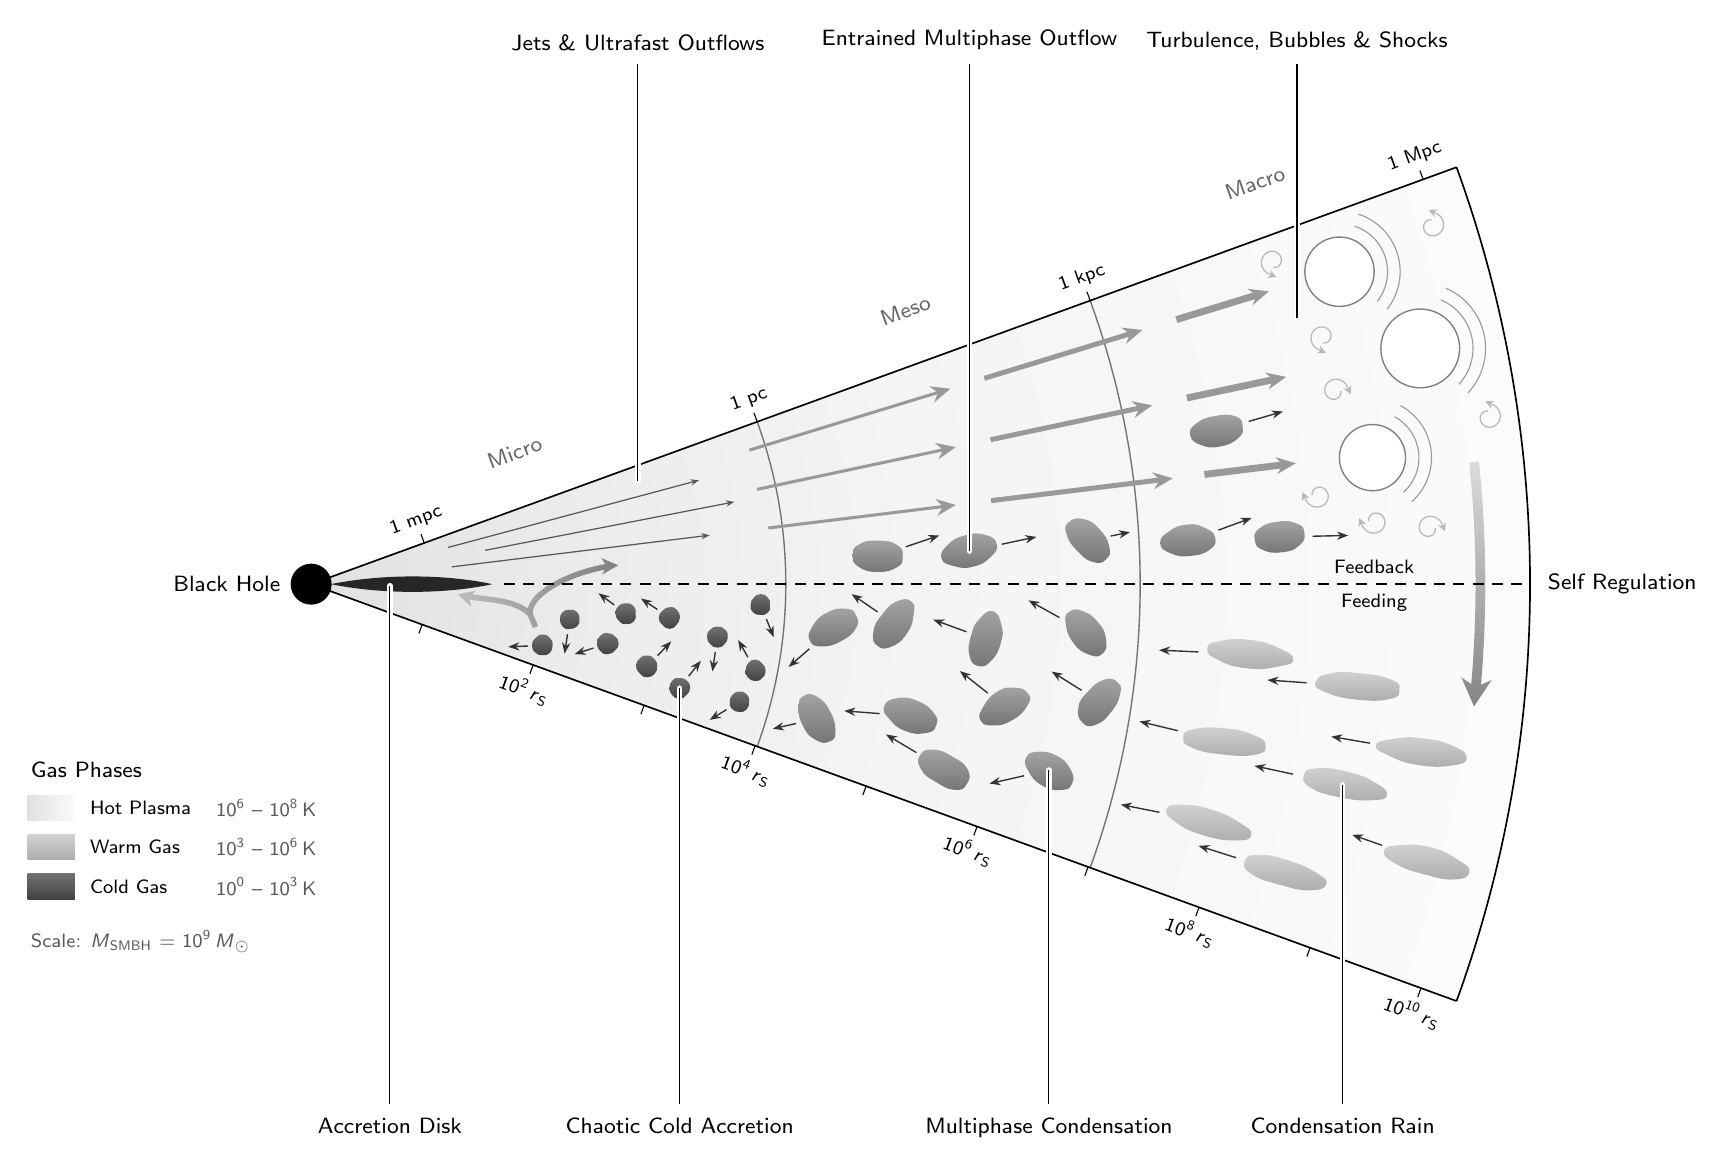
\begin{tikzpicture}[font=\footnotesize]

% wedge filled with the hot halo plasma
\begin{scope}
  \clip (0,0) -- (\half:\smax*\L) arc[start angle=\half,end angle=-\half,radius=\smax*\L] -- cycle;
  \shade[shading=halo] (0,0) circle (\smax*\L);
\end{scope}

% scale zones bounded by arcs at 1 pc and 1 kpc
\foreach \s in {\spc,\skpc}
  \draw[line width=0.5pt,zonec] ({\half}:{(\s)*\L}) arc[start angle=\half,end angle=-\half,radius=\s*\L];

% feeding, lower half
\pgfmathsetseed{1}
\foreach \s/\a/\r/\d/\st/\l in \rainlist{
  \begin{scope}[shift={({\a}:{(\s)*\L})}]\cloud{0.55}{0.17}{\r}{warm}\end{scope}
  \move{({\a}:{(\s)*\L})}{\d}{\st}{\l}
}
\pgfmathsetseed{2}
\foreach \s/\a/\r/\d/\st/\l in \mesoinlist{
  \begin{scope}[shift={({\a}:{(\s)*\L})}]\cloud{0.34}{0.2}{\r}{multi}\end{scope}
  \move{({\a}:{(\s)*\L})}{\d}{\st}{\l}
}
\pgfmathsetseed{3}
\foreach \s/\a/\r/\d/\st/\l in \ccalist{
  \begin{scope}[shift={({\a}:{(\s)*\L})}]\cloud{0.13}{0.13}{0}{cold}\end{scope}
  \move{({\a}:{(\s)*\L})}{\d}{\st}{\l}
}

% accretion disk around the black hole
\shade[left color=diskA,right color=diskB] (0.25,0) .. controls (1.0,0.15) and (1.8,0.11) .. (2.3,0)
  .. controls (1.8,-0.11) and (1.0,-0.15) .. (0.25,0) -- cycle;
% gas from the innermost clump splits, part accretes onto the disk, part powers the feedback,
% written as one outline of stem, branches and heads so the whole fork carries one gradient
\shade[fork]
  (2.036,-0.286) -- (1.860,-0.130) -- (2.091,-0.083) -- (2.043,-0.129) -- (2.348,-0.169)
  -- (2.425,-0.182) -- (2.501,-0.199) -- (2.573,-0.220) -- (2.643,-0.247) -- (2.698,-0.275)
  -- (2.751,-0.309) -- (2.761,-0.277) -- (2.778,-0.239) -- (2.800,-0.204) -- (2.827,-0.168)
  -- (2.858,-0.134) -- (2.894,-0.101) -- (2.976,-0.037) -- (3.053,0.012) -- (3.137,0.059)
  -- (3.227,0.101) -- (3.322,0.141) -- (3.419,0.176) -- (3.537,0.211) -- (3.636,0.236)
  -- (3.736,0.256) -- (3.683,0.332) -- (3.900,0.240) -- (3.696,0.122) -- (3.728,0.183)
  -- (3.632,0.163) -- (3.537,0.138) -- (3.441,0.109) -- (3.347,0.075) -- (3.238,0.029)
  -- (3.152,-0.013) -- (3.058,-0.066) -- (2.989,-0.114) -- (2.929,-0.163) -- (2.881,-0.213)
  -- (2.845,-0.263) -- (2.826,-0.302) -- (2.816,-0.340) -- (2.815,-0.372) -- (2.882,-0.531)
  -- (2.818,-0.559) -- (2.750,-0.400) -- (2.716,-0.371) -- (2.672,-0.341) -- (2.624,-0.316)
  -- (2.562,-0.290) -- (2.471,-0.264) -- (2.375,-0.244) -- (2.274,-0.229) -- (2.010,-0.196) -- cycle;

% feedback, upper half
% jets and ultrafast outflows launched close to the black hole
% at angle a from s0 to s1, the middle one set back so the three are not packed together
\foreach \a/\sa/\sb in {7/1.2/3.4,11/1.5/3.65,15/1.2/3.4}
  \draw[-{Stealth[length=3pt]},line width=0.45pt,jetc] ({\a}:{\sa*\L}) -- ({\a}:{\sb*\L});
% broad outflow widening outwards in three stages, a and the start and end s of each stage,
% the first stages cross the 1 pc arc and end together, leaving a corridor for the entrained pointer
\foreach \a/\sa/\sb/\sc/\sd/\se/\sf in {
    7/3.9/5.5/5.8/7.35/7.62/8.4,
    12/3.86/5.58/5.88/7.28/7.58/8.44,
    17/3.88/5.66/5.96/7.36/7.66/8.48}{
  \draw[outflow,line width=1.1pt] ({\a}:{\sa*\L}) -- ({\a}:{\sb*\L});
  \draw[outflow,line width=1.8pt] ({\a}:{\sc*\L}) -- ({\a}:{\sd*\L});
  \draw[outflow,line width=2.5pt] ({\a}:{\se*\L}) -- ({\a}:{\sf*\L});
}
\pgfmathsetseed{4}
\foreach \s/\a/\r/\d/\st/\l in \mesooutlist{
  \begin{scope}[shift={({\a}:{(\s)*\L})}]\cloud{0.34}{0.2}{\r}{multi}\end{scope}
  \move{({\a}:{(\s)*\L})}{\d}{\st}{\l}
}
% bubbles inflated at the ends of the outflow streams, s, a and radius, emptied of hot plasma so
% they are left nearly white, each driving two shock
% fronts into the halo on its outer side
\foreach \s/\a/\r [count=\k] in {9.05/6.8/0.42,9.6/12.0/0.5,9.1/16.9/0.44}{
  \coordinate (bub\k) at ({\a}:{(\s)*\L});
  \shade[inner color=bubfill,outer color=bubedge] (bub\k) circle (\r);
  \draw[bubline,line width=0.5pt] (bub\k) circle (\r);
  \foreach \dr in {0.17,0.33}
    \draw[shockc,line width=0.4pt] ($(bub\k)+(\a-55:\r+\dr)$)
      arc[start angle=\a-55,end angle=\a+55,radius=\r+\dr];
}
% turbulent eddies stirred up around the bubbles, small spirals widening outwards, given by centre,
% outer radius, start angle and the angle turned, negative for clockwise, the head continues the
% spiral along its tangent from the outer end
\foreach \x/\y/\r/\b/\t in {
    13.00/2.45/0.17/0/-340,
    14.23/4.55/0.17/90/340,
    12.79/1.13/0.17/180/-340,
    12.85/3.14/0.17/270/340,
    14.20/0.71/0.17/0/-340,
    14.95/2.12/0.17/90/340,
    13.51/0.80/0.17/180/-340,
    12.22/4.10/0.17/270/340}{
  \draw[eddy] plot[smooth,domain=0:\t,samples=36,variable=\u]
    ({\x+\r*(0.45+0.55*\u/\t)*cos(\b+\u)},{\y+\r*(0.45+0.55*\u/\t)*sin(\b+\u)});
  \pgfmathsetmacro{\e}{\t+4*sign(\t)}
  \coordinate (q0) at ({\x+\r*cos(\b+\t)},{\y+\r*sin(\b+\t)});
  \coordinate (q1) at ({\x+\r*(0.45+0.55*\e/\t)*cos(\b+\e)},{\y+\r*(0.45+0.55*\e/\t)*sin(\b+\e)});
  \draw[eddy,-{Stealth[length=3pt,width=3pt]}] (q0) -- ($(q0)!3pt!(q1)$);
}

% self regulation, the feedback heats the halo and the halo cools back into the feeding rain
\shade[cycle]
  ({6}:{\rreg+0.062}) arc[start angle=6,end angle=-4.92,radius=\rreg+0.062]
  -- ({-4.64}:{\rreg+0.193}) -- ({-6}:{\rreg}) -- ({-4.64}:{\rreg-0.193})
  -- ({-4.92}:{\rreg-0.062}) arc[start angle=-4.92,end angle=6,radius=\rreg-0.062] -- cycle;

% black hole
\fill[black] (0,0) circle (0.26);

% wedge outline, midline between feedback and feeding, and decade ticks on both edges
\draw[line width=0.6pt] (\half:\smax*\L) -- (0,0) -- (-\half:\smax*\L);
\draw[line width=0.6pt] (\half:\smax*\L) arc[start angle=\half,end angle=-\half,radius=\smax*\L];
\draw[line width=0.5pt,dash pattern=on 4pt off 3pt] (2.45,0) -- (\smax*\L,0);
\foreach \s in {1,...,10}
  \draw[line width=0.4pt] ({-\half}:{\s*\L}) -- ++(-\half-90:0.12);
\foreach \s in {\smpc,\spc,\skpc,\sMpc}
  \draw[line width=0.4pt] ({\half}:{(\s)*\L}) -- ++(\half+90:0.12);

% scale labels, r over r_S along the lower edge and physical radius along the upper edge
\foreach \s in {2,4,6,8,10}{
  \coordinate (m) at ({-\half}:{\s*\L});
  \node[edge,rotate=-\half,anchor=north] at ($(m)+(-\half-90:0.12)$) {\dec{\s}\,\rs};}
\foreach \s/\u in {\smpc/1 mpc,\spc/1 pc,\skpc/1 kpc,\sMpc/1 Mpc}{
  \coordinate (m) at ({\half}:{(\s)*\L});
  \node[edge,rotate=\half,anchor=south] at ($(m)+(\half+90:0.12)$) {\u};}
% scale zones named along the upper edge
\foreach \s/\z in {2.0/Micro,5.52/Meso,8.67/Macro}{
  \coordinate (m) at ({\half}:{\s*\L});
  \node[lab,text=zonetext,rotate=\half,anchor=south] at ($(m)+(\half+90:0.55)$) {\z};}

% feedback and feeding named along the midline, self regulation named beside its arrow
\node[lab,font=\scriptsize,anchor=south,inner sep=3.5pt] at ({0}:{9.0*\L}) {Feedback};
\node[lab,font=\scriptsize,anchor=north,inner sep=3.5pt] at ({0}:{9.0*\L}) {Feeding};
\node[lab,anchor=west,inner sep=2pt] at ({0}:{\smax*\L+0.15}) {Self Regulation};

% component labels in two aligned rows with vertical pointers, labels naming several
% components point at the background between them
\toplabel{(4.15,1.31)}{Jets \& Ultrafast Outflows}
\toplabel{(8.36,0.42)}{Entrained Multiphase Outflow}
\toplabel{(12.52,3.38)}{Turbulence, Bubbles \& Shocks}
\botlabel{(1.00,-0.02)}{Accretion Disk}
\botlabel{(4.68,-1.32)}{Chaotic Cold Accretion}
\botlabel{(9.37,-2.36)}{Multiphase Condensation}
\botlabel{(13.10,-2.55)}{Condensation Rain}
\node[lab,anchor=east] at (-0.35,0) {Black Hole};

% legend of the gas phases
\begin{scope}[shift={(-3.6,-2.6)}]
  \node[lab,anchor=south west] at (0,0.1) {Gas Phases};
  \shade[left color=halo0,right color=halo3] (0,-0.4) rectangle ++(0.6,0.32);
  \path[warm] (0,-0.9) rectangle ++(0.6,0.32);
  \path[cold] (0,-1.4) rectangle ++(0.6,0.32);
  \foreach \txt/\T [count=\n from 0] in
      {Hot Plasma/{\dec{6} -- \dec{8}},Warm Gas/{\dec{3} -- \dec{6}},Cold Gas/{\dec{0} -- \dec{3}}}{
    \node[lab,font=\scriptsize,anchor=west] at (0.75,-\n*0.5-0.24) {\txt};
    \node[lab,font=\scriptsize,anchor=west,text=legtext] at (2.35,-\n*0.5-0.24) {\T\,K};
  }
  \node[lab,font=\scriptsize,anchor=north west,text=legtext] at (0,-1.75)
    {Scale: \textit{M}\textsubscript{SMBH} = \dec{9}\,\msun};
\end{scope}

\end{tikzpicture}
\end{document}
